\documentclass[a4paper,12pt,oneside]{article}

\usepackage[utf8]{inputenc}
\usepackage[T2A]{fontenc}
\usepackage[russian]{babel}
\usepackage[usenames]{xcolor}
\usepackage{etoolbox}
\usepackage{listings}
\usepackage{graphicx}
\usepackage{cmap}
\usepackage{indentfirst}
\usepackage{makeidx}
\usepackage[unicode]{hyperref}

\newif\ifanswers
\answerstrue

\hypersetup{
%bookmarks=true,            % show bookmarks bar?
%unicode=false,             % non-Latin characters in Acrobat’s bookmarks
pdfproducer={Producer},    % producer of the document
pdfkeywords={keywords},    % list of keywords
pdfnewwindow=true,         % links in new window
colorlinks=true,           % false: boxed links; true: colored links
linkcolor=black,           % color of internal links
citecolor=black,           % color of links to bibliography
    filecolor=black,           % color of file links
    urlcolor=black             % color of external links
}

\renewcommand{\rmdefault}{cmr} 

\renewcommand{\texttt}[2][black]{\textcolor{#1}{\ttfamily #2}}

\definecolor{OliveGreen}{cmyk}{0.64,0,0.95,0.40}
\definecolor{mauve}{rgb}{0.58,0,0.82}

\setlength{\parskip}{6pt}

\makeindex

\title{Лекция по Toolchain}
\author{
  Владимиров Константин Игоревич\\
  \texttt{konstantin.vladimirov@gmail.com}
}
\date{\today}

\lstset{
language=C++,                           % Code langugage
basicstyle=\ttfamily,                   % Code font, Examples: \footnotesize, \ttfamily
keywordstyle=\color{OliveGreen},        % Keywords font ('*' = uppercase)
commentstyle=\color{gray},              % Comments font
stringstyle=\color{mauve},
numbers=left,                           % Line nums position
numberstyle=\tiny,
numbersep=10pt,
stepnumber=1,                           % Step between two line-numbers
frame=none,                             % A frame around the code
tabsize=2,                              % Default tab size
captionpos=b,                           % Caption-position = bottom
breaklines=true,                        % Automatic line breaking?
breakatwhitespace=false,                % Automatic breaks only at whitespace?
showspaces=false,                       % Dont make spaces visible
showstringspaces=false,
showtabs=false,                         % Dont make tabls visible
columns=flexible,                       % Column format
title=\lstname,
caption={},
extendedchars=\true,
inputencoding=utf8,
}

\begin{document}

\section{Toolchain}\label{Toolchain}

\subsection{Введение}\label{Introduction}

Общеупотребительным англицизмом toolchain (можно перевести как ``набор средств разработки'' или как ``система компиляции'', можно оставить просто слово ``тулчейн'') обозначают набор средств разработки, совместно используемых для создания программного обеспечения. Обычно это компилятор, ассемблер, линкер, а также набор бинарных утилит. Иногда в состав toolchain включают средства отладки и верификации программ, профилировщики и анализаторы покрытия кода.

Обычно весь набор средств разработки скрыт от пользователя за единой программой-драйвером (как в случае GNU Toolchain когда роль такой программы играет GCC) или за ширмой средств IDE (как в случае Microsoft Toolchain, когда компиляция ассемблирование и сборка происходят по нажатию кнопки F7 в Visual Studio).

Кроме GNU и Microsoft, известны также LLVM toolchain, Intel toolchain, ARM toolchain а также пакеты средств разработки Borland и Comeau. Для всех примеров ниже будет использоваться GNU Toolchain, но иногда будут приводиться примеры из других средств разработки, там, где есть некие концептуальные отличия. Точно также ниже будут описаны в основном примеры компиляции программ на языке C, разве что с некоторыми экскурсиями в C++ и Fortran.

Эта лекция ставит перед собой следующие цели:

\begin{itemize}
\item Сделать ясной структуру и последовательность работы системы компиляции в целом
\item Осветить роль каждого из инструментов в отдельности, его применимость и решаемые им задачи
\item Дать базу для самостоятельных экспериментов (на примере GNU Toolchain)
\item Изложить основные этапы портирования toolchain на новую архитектуру
\end{itemize}

Первый пункт можно переформулировать как простой и конкретный вопрос: что происходит при исполнении строчки вида

\begin{verbatim}
$ gcc test.c
\end{verbatim}

Правильный ответ: происходит запуск трёх основных программ, как это показано на (рис. \ref{fig:simplified_scheme}).

\begin{figure}[ht]
\centering
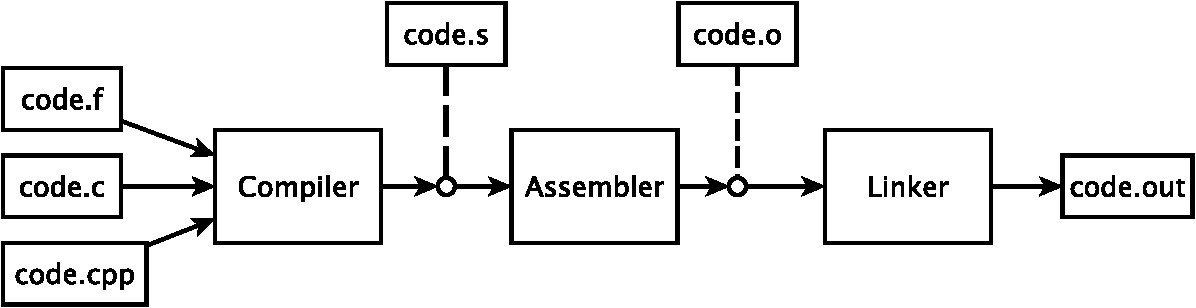
\includegraphics[width=1.0\textwidth]{illustrations/simplified-scheme-crop.pdf}
\caption{Упрощенная схема toolchain}
\label{fig:simplified_scheme}
\end{figure}

\begin{enumerate}
\item \textbf{Компилятор} -- в случае GNU toolchain это cc1 или cc1plus для кода на C или C++, в случае MSVS это cl.exe. Переводит текст на языке высокого уровня в язык ассемблера целевой архитектуры
\item \textbf{Ассемблер} -- в случае GNU toolchain это as, в случае MSVS это ml.exe. Кодирует ассемблер целевой архитектуры и порождает объектный код
\item \textbf{Линкер} -- в случае GNU toolchain это ld или gold, в случае MSVS это link.exe. Собирает несколько объектных модулей в исполняемый файл
\end{enumerate}

Toolchain не исчерпывается этой упрощенной схемой, но для начала рассмотрение трёх основных компонент позволяет создать общую картину происходящего.

\subsection{Компилятор}

Компилятор является главным и наиболее известным компонентом средств разработки (автору не раз доводилось слышать как ``компилятором'' называют и драйвер и весь toolchain). Тем не менее, происходящее внутри компилятора часто также остается неизвестным разработчику, как и происходящее внутри системы компиляции в целом.

\begin{figure}[ht]
\centering
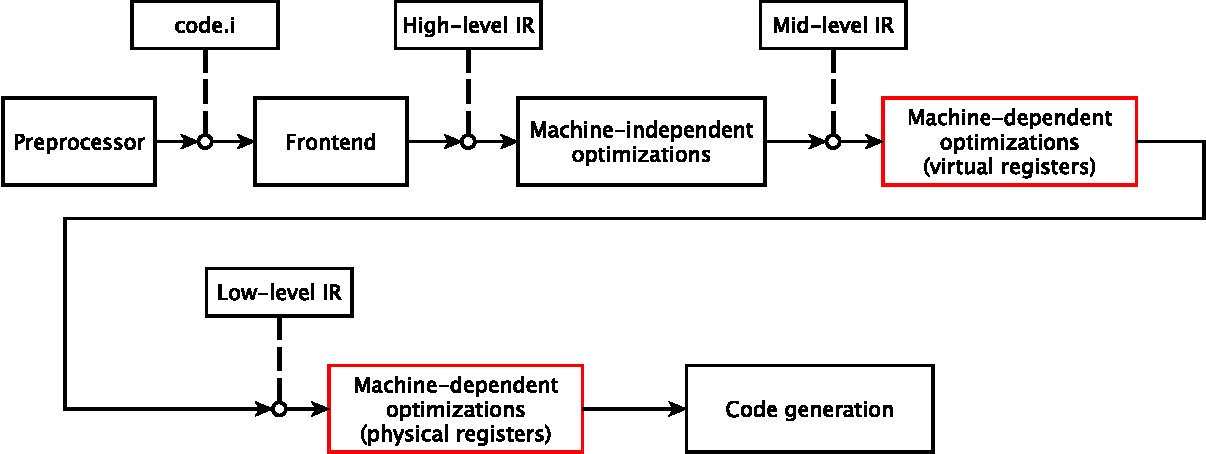
\includegraphics[width=1.0\textwidth]{illustrations/compiler-crop.pdf}
\caption{Компилятор изнутри}
\label{fig:compiler_scheme}
\end{figure}

На (рис. \ref{fig:compiler_scheme}) изображена схема работы компилятора, состоящая из следующих элементов:

\begin{enumerate}
\item \textbf{Препроцессор} -- занимается текстовой обработкой исходного текста и подготовкой к компиляции
\item \textbf{Фронтенд} -- переводит язык высокого уровня в промежуточное представление
\item \textbf{Бэкенд} -- состоит из оптимизаций на разных уровнях промежуточного представления и кодогенерации в ассемблер целевой архитектуры. Иногда его делят на middle-end, где выполняются машинно-независимые оптимизации и backend (выделен красным цветом), где происходят машинно-зависимые преобразования.
\end{enumerate}

В LLVM toolchain, препроцессор и фронтенд вынесены в отдельную программу (clang), которая порождает машинно-независимое промежуточное представление (intermediate representation или для краткости IR) над которым сосбтвенно компилятор llvm производит преобразования до ассемблера. Кроме того собственно препроцессор часто поставляет отдельно в наборе бинарных утилит, например в составе GNU Toolchain программа, производящая препроцессинг называется cpp. Она, тем не менее, не запускается в нормальной циклограмме работы, так как препроцессор является частью компилятора cc1, а cpp это просто отдельно лежащий препроцессор, отпиленный для удобства.

\subsubsection{Препроцессор}

Работа препроцессора происходит в основном над текстом и в случае языка C регламентирована стандартом языка (5.1.1.2 в C11). В случае gcc, для препроцессирования файла имеется опция -E.

Препроцессор выполняет действия в следующем порядке:
\begin{itemize}
\item Замена триграфов.
Например попробуйте понять что происходит на этой строчке: \lstinline$!ErrorOccured() ??!??! HandleError();$. Правильный ответ -- здесь вместо вертикальной черты использован триграф \lstinline$??!$ так что непонятная мешанина знаков в середине это просто длинное или. Ещё пример: 

\begin{lstlisting}
// WTF????/
a += 1;
\end{lstlisting}

Здесь использован триграф \lstinline$??/$, обозначающий обратный слеш. Что приводит к следующему пункту.
\item Объединение строк по обратному слешу
В примере выше после раскрытия триграфа остаётся:
\begin{lstlisting}
// WTF??\
a += 1;
\end{lstlisting}
И на этом этапе эти строки будут объединены в:
\begin{lstlisting}
// WTF??a += 1;
\end{lstlisting}
\item Разбиение на токены препроцессирования и замена комментариев пробелами
Здесь будут вычеркнуты все комментарии и заменены одним пробельным символом.
\item Раскрытие макросов и обработка директив препроцессора
На этом этапе раскрываются все макро-определения, как явно введенные через директиву \lstinline!#define! так и неявно заданные как билтины компилятора (скажем \lstinline!__cplusplus! позволяющий отличить компиляцию на C и C++). В случае GNU Toolchain, посмотреть встроенные макроопределения можно с помощью опций -E -dM.
\item Замена escape-последовательностей
Я полагаю, все встречались со \lstinline!\n! или \lstinline!\t! при использовании функции \lstinline!printf!
\item Соединение стоящих рядом строковых литералов
\end{itemize}

Файл, получившийся после препроцессирования,

\end{document}
